% Current collaborator review, exported on 2026-10-13 from the Markdown note.
% Source SHA256: 1bd9a1c377610e8f45e178b48633a1c887f5ab5f895980bd75021753e3ac6314
% Conversion: Pandoc 3.6.2; markdown+tex_math_single_backslash -> standalone LaTeX;
% xelatex engine, geometry:margin=20mm, fontsize=10pt, colorlinks=true.
% Text Unicode symbols are mapped to equivalent LaTeX commands for portability.
% Compile from docs/research: xelatex location_only_meeting_brief.tex (twice).
% TeX compilation was not available on the export host; no PDF build is claimed.
% The Markdown document remains the canonical editable summary.
% Options for packages loaded elsewhere
\PassOptionsToPackage{unicode}{hyperref}
\PassOptionsToPackage{hyphens}{url}
\PassOptionsToPackage{dvipsnames,svgnames,x11names}{xcolor}
\documentclass[
  10pt,
]{article}
\usepackage{xcolor}
\usepackage[margin=20mm]{geometry}
\usepackage{amsmath,amssymb}
\setcounter{secnumdepth}{-\maxdimen} % remove section numbering
\usepackage{iftex}
\ifPDFTeX
  \usepackage[T1]{fontenc}
  \usepackage[utf8]{inputenc}
  \usepackage{textcomp} % provide euro and other symbols
\else % if luatex or xetex
  \usepackage{unicode-math} % this also loads fontspec
  \defaultfontfeatures{Scale=MatchLowercase}
  \defaultfontfeatures[\rmfamily]{Ligatures=TeX,Scale=1}
\fi
\usepackage{lmodern}
\ifPDFTeX\else
  % xetex/luatex font selection
\fi
% Use upquote if available, for straight quotes in verbatim environments
\IfFileExists{upquote.sty}{\usepackage{upquote}}{}
\IfFileExists{microtype.sty}{% use microtype if available
  \usepackage[]{microtype}
  \UseMicrotypeSet[protrusion]{basicmath} % disable protrusion for tt fonts
}{}
\makeatletter
\@ifundefined{KOMAClassName}{% if non-KOMA class
  \IfFileExists{parskip.sty}{%
    \usepackage{parskip}
  }{% else
    \setlength{\parindent}{0pt}
    \setlength{\parskip}{6pt plus 2pt minus 1pt}}
}{% if KOMA class
  \KOMAoptions{parskip=half}}
\makeatother
\usepackage{color}
\usepackage{fancyvrb}
\newcommand{\VerbBar}{|}
\newcommand{\VERB}{\Verb[commandchars=\\\{\}]}
\DefineVerbatimEnvironment{Highlighting}{Verbatim}{commandchars=\\\{\}}
% Add ',fontsize=\small' for more characters per line
\newenvironment{Shaded}{}{}
\newcommand{\AlertTok}[1]{\textcolor[rgb]{1.00,0.00,0.00}{\textbf{#1}}}
\newcommand{\AnnotationTok}[1]{\textcolor[rgb]{0.38,0.63,0.69}{\textbf{\textit{#1}}}}
\newcommand{\AttributeTok}[1]{\textcolor[rgb]{0.49,0.56,0.16}{#1}}
\newcommand{\BaseNTok}[1]{\textcolor[rgb]{0.25,0.63,0.44}{#1}}
\newcommand{\BuiltInTok}[1]{\textcolor[rgb]{0.00,0.50,0.00}{#1}}
\newcommand{\CharTok}[1]{\textcolor[rgb]{0.25,0.44,0.63}{#1}}
\newcommand{\CommentTok}[1]{\textcolor[rgb]{0.38,0.63,0.69}{\textit{#1}}}
\newcommand{\CommentVarTok}[1]{\textcolor[rgb]{0.38,0.63,0.69}{\textbf{\textit{#1}}}}
\newcommand{\ConstantTok}[1]{\textcolor[rgb]{0.53,0.00,0.00}{#1}}
\newcommand{\ControlFlowTok}[1]{\textcolor[rgb]{0.00,0.44,0.13}{\textbf{#1}}}
\newcommand{\DataTypeTok}[1]{\textcolor[rgb]{0.56,0.13,0.00}{#1}}
\newcommand{\DecValTok}[1]{\textcolor[rgb]{0.25,0.63,0.44}{#1}}
\newcommand{\DocumentationTok}[1]{\textcolor[rgb]{0.73,0.13,0.13}{\textit{#1}}}
\newcommand{\ErrorTok}[1]{\textcolor[rgb]{1.00,0.00,0.00}{\textbf{#1}}}
\newcommand{\ExtensionTok}[1]{#1}
\newcommand{\FloatTok}[1]{\textcolor[rgb]{0.25,0.63,0.44}{#1}}
\newcommand{\FunctionTok}[1]{\textcolor[rgb]{0.02,0.16,0.49}{#1}}
\newcommand{\ImportTok}[1]{\textcolor[rgb]{0.00,0.50,0.00}{\textbf{#1}}}
\newcommand{\InformationTok}[1]{\textcolor[rgb]{0.38,0.63,0.69}{\textbf{\textit{#1}}}}
\newcommand{\KeywordTok}[1]{\textcolor[rgb]{0.00,0.44,0.13}{\textbf{#1}}}
\newcommand{\NormalTok}[1]{#1}
\newcommand{\OperatorTok}[1]{\textcolor[rgb]{0.40,0.40,0.40}{#1}}
\newcommand{\OtherTok}[1]{\textcolor[rgb]{0.00,0.44,0.13}{#1}}
\newcommand{\PreprocessorTok}[1]{\textcolor[rgb]{0.74,0.48,0.00}{#1}}
\newcommand{\RegionMarkerTok}[1]{#1}
\newcommand{\SpecialCharTok}[1]{\textcolor[rgb]{0.25,0.44,0.63}{#1}}
\newcommand{\SpecialStringTok}[1]{\textcolor[rgb]{0.73,0.40,0.53}{#1}}
\newcommand{\StringTok}[1]{\textcolor[rgb]{0.25,0.44,0.63}{#1}}
\newcommand{\VariableTok}[1]{\textcolor[rgb]{0.10,0.09,0.49}{#1}}
\newcommand{\VerbatimStringTok}[1]{\textcolor[rgb]{0.25,0.44,0.63}{#1}}
\newcommand{\WarningTok}[1]{\textcolor[rgb]{0.38,0.63,0.69}{\textbf{\textit{#1}}}}
\usepackage{longtable,booktabs,array}
\usepackage{calc} % for calculating minipage widths
% Correct order of tables after \paragraph or \subparagraph
\usepackage{etoolbox}
\makeatletter
\patchcmd\longtable{\par}{\if@noskipsec\mbox{}\fi\par}{}{}
\makeatother
% Allow footnotes in longtable head/foot
\IfFileExists{footnotehyper.sty}{\usepackage{footnotehyper}}{\usepackage{footnote}}
\makesavenoteenv{longtable}
\usepackage{graphicx}
\makeatletter
\newsavebox\pandoc@box
\newcommand*\pandocbounded[1]{% scales image to fit in text height/width
  \sbox\pandoc@box{#1}%
  \Gscale@div\@tempa{\textheight}{\dimexpr\ht\pandoc@box+\dp\pandoc@box\relax}%
  \Gscale@div\@tempb{\linewidth}{\wd\pandoc@box}%
  \ifdim\@tempb\p@<\@tempa\p@\let\@tempa\@tempb\fi% select the smaller of both
  \ifdim\@tempa\p@<\p@\scalebox{\@tempa}{\usebox\pandoc@box}%
  \else\usebox{\pandoc@box}%
  \fi%
}
% Set default figure placement to htbp
\def\fps@figure{htbp}
\makeatother
\setlength{\emergencystretch}{3em} % prevent overfull lines
\providecommand{\tightlist}{%
  \setlength{\itemsep}{0pt}\setlength{\parskip}{0pt}}
\usepackage{bookmark}
\IfFileExists{xurl.sty}{\usepackage{xurl}}{} % add URL line breaks if available
\urlstyle{same}
\hypersetup{
  colorlinks=true,
  linkcolor={Maroon},
  filecolor={Maroon},
  citecolor={Blue},
  urlcolor={Blue},
  pdfcreator={LaTeX via pandoc}}

\author{}
\date{}

\begin{document}

\section{Location-only inference: collaborator review
note}\label{location-only-inference-collaborator-review-note}

12 October 2026 \textperiodcentered{} For discussion with Christian Robert and Antoine.

This is the current technical account of the known-scale location work.
It explains the target, the implemented corrections, and the evidence
needed to judge them. It replaces the earlier smoke-study brief at this
path. The previous version is preserved in the
\href{evidence/location_review_handoff_2026-10-12/documents_before.tar.gz}{document
snapshot}. The \href{../paper/paper.tex}{LaTeX manuscript} remains an
earlier draft; its results and figures have not been brought up to this
review's scope.

\subsection{1. Where we stand}\label{where-we-stand}

We infer a location parameter from a released \textbf{selected global
MLE}. Student-t is the main model. Logistic and Laplace are comparators.
Scale is known.

We have corrected the statistical target and implemented several valid
kernels on their stated regular domains. We also have independent
simulation references. These are distinct achievements from
demonstrating good mixing. The latest saved chains show that a sound
RATTLE acceptance rule can coexist with slow latent-data exploration.
Agreement of parameter means is not sufficient validation.

\begin{longtable}[]{@{}
  >{\raggedright\arraybackslash}p{(\linewidth - 2\tabcolsep) * \real{0.5000}}
  >{\raggedright\arraybackslash}p{(\linewidth - 2\tabcolsep) * \real{0.5000}}@{}}
\toprule\noalign{}
\begin{minipage}[b]{\linewidth}\raggedright
Method
\end{minipage} & \begin{minipage}[b]{\linewidth}\raggedright
Current evidence and use
\end{minipage} \\
\midrule\noalign{}
\endhead
\bottomrule\noalign{}
\endlastfoot
Student corrected pair Gibbs & Transparent correctness baseline; earlier
reference checks pass. Expensive; outside the latest timing
comparison. \\
Student reversible-block Gibbs & All three latest cases pass reference
and expanded latent checks. Practical constrained method, especially for
shifted-prior latent tails. \\
Student selected RATTLE & Corrected regular-region target. All three
latest cases have reference or latent-mixing warnings. \\
Student independence MH & All three latest cases pass bulk and 5\%/95\%
checks. Shifted case is slower and has limited outer-1\% precision. \\
Logistic block Gibbs / RATTLE & Block passes three cases, one
borderline. RATTLE passes only one of three expanded checks; labelled
observations mix slowly at n=10. \\
Laplace median Gibbs / facet HMC & Both pass all four tested cases.
Gibbs is faster; direct simulation is cheaper still. \\
Affine sampler & Valid location-equivariance construction with prior
validation. Recorded shifted-case latent-mixing problems; not retimed in
this study. \\
Raw weighted MC / prior rejection & Independent reference construction /
independent posterior draws. Efficiency depends on prior overlap. \\
\end{longtable}

``Pass'' refers to finite, declared checks, not universal convergence.
Legacy score samplers remain separate comparators. Joint location-scale
methods are still experimental; \texttt{models/scale/} is a placeholder.
The \href{../../models/README.md}{model guide} identifies current
imports and legacy aliases.

\subsection{2. The distribution we condition
on}\label{the-distribution-we-condition-on}

Let \(F_\mu(x)=\prod_i f_0(x_i-\mu)\), let \(\pi_0\) be the prior, and
let \(t=T(x)\) be the released statistic. For Student data, \(T\)
selects the global likelihood maximizer and chooses the smaller location
only for an exact tie. Logistic has a unique location maximum. For
Laplace we select the middle observation at odd n and the midpoint of
the two middle observations at even n.

For unit-scale Student data, define

\[
\psi(y)=\frac{y}{k+y^2},\quad C(x)=\sum_i\psi(x_i-t),\quad
J(x)=\sum_i\psi'(x_i-t),\quad G(x)=\sum_i\psi'(x_i-t)^2.
\]

Relative to surface measure on the regular score-zero manifold, the
joint score-conditioned and selected-MLE targets are respectively

\[
\rho_C(\mu,x)\propto\pi_0(\mu)\frac{F_\mu(x)}{\sqrt{G(x)}},
\qquad
\rho_T(\mu,x)\propto\pi_0(\mu)\frac{F_\mu(x)}{\sqrt{G(x)}}W(x),
\] \[
W(x)=\mathbf1\{T(x)=t\}|J(x)|.
\]

On a smooth estimator branch, implicit differentiation gives
\(\nabla_xT=\nabla_xC/J\). Coarea then gives the extra factor \(|J|\).
At a nondegenerate selected maximum, \(J>0\). This establishes both
required corrections: global selection and curvature. Score zero can be
a local minimum or an inferior local maximum; positive curvature alone
is insufficient.

These formulas concern regular regions, with common normalization of the
joint law. One cannot normalize the latent conditional separately at
each \(\mu\) and then retain the original prior without accounting for
that normalization. Singular roots and tie boundaries need separate
treatment. Floating-point constraint tolerances approximate this
mathematical fiber; they do not make it an exact algebraic identity.

The two targets coincide if their supports agree up to null sets and
\(W\) is constant almost everywhere under the score-conditioned law.
Known-variance Gaussian location is the basic example. A unique score
root, as in Logistic, does \textbf{not} make the curvature factor
constant. Because \(W\) depends only on \(x\), the ordinary parameter
update \(p(\mu\mid x)\) remains valid. See the
\href{selected_mle_target_audit.md}{target audit} for the full
derivation; its descriptions of then-current uncorrected code are
historical findings.

\subsection{3. What we corrected in Gibbs and
RATTLE}\label{what-we-corrected-in-gibbs-and-rattle}

\subsubsection{Student Gibbs: correct the joint pair, or a reversible
block}\label{student-gibbs-correct-the-joint-pair-or-a-reversible-block}

Write \(z_i=\psi(x_i-t)\). A pair update preserves \(z_i+z_j=\delta\).
Away from zero and the branch folds, each score coordinate has two
finite inverse branches. Their weights must include the inverse
Jacobian:

\[
w_\mu(z,b)=\frac{f_k(t+y_b(z)-\mu)}{|\psi'(y_b(z))|},\qquad
q_\mu(z)=\sum_b w_\mu(z,b).
\]

The transparent corrected pair method proposes \(z_i'\), sets
\(z_j'=\delta-z_i'\), and draws both branches with probabilities
\(w/q\). The branch terms cancel in the \textbf{joint} MH ratio, leaving

\[
\log r=\log\frac{q_\mu(z_i')q_\mu(z_j')}{q_\mu(z_i)q_\mu(z_j)}
+\log\frac{h(z_i\mid z_i')}{h(z_i'\mid z_i)}
+\log W(x')-\log W(x).
\]

The entire joint proposal is accepted or rejected. Refreshing a branch
after this rejection would invalidate that argument. Merely changing
branch weights would leave the score-coordinate update uncorrected.

The faster method holds \(\mu\) fixed and makes a fixed number \(m\) of
uniform random-scan pair moves. Each score-target pair kernel is
reversible; its random-scan mixture \(K\), and hence \(K^m\), are
reversible. A single outer acceptance \(\min(1,W(x')/W(x))\) therefore
gives the selected target. Indeed, the accepted flow is proportional to
\(\rho_C(x)K^m(x,dx')\min(W(x),W(x'))\), which is symmetric. An
arbitrary ordered sweep does not have this guarantee.

This uses a \textbf{separate compiled regular-region pair kernel}, not
an unchanged legacy sweep. The audit found finite-strip cutoffs,
derivative floors, approximate/clipped inverse-CDF proposals, and silent
fallback behavior in the legacy machinery. The corrected kernel removes
those target-changing rules, uses the proper truncated proposal and
Hastings normalizer, and reports unresolved numerical cases. The later
update also fixes cancellation in the truncated-normal normalizer and
uses an unfloored MH uniform for selected parameter updates. The
mathematical parameter conditional is unchanged.

Within a score pair move, refreshing branches after rejection of the
\emph{scalar} score proposal is valid: it is the conditional branch draw
for the retained score coordinates. Rejection of the \emph{outer
selected block} restores the whole previous latent state. These are
different rejection events. Intermediate block states may be
MLE-invalid; only the endpoint needs the selected support test. Cheap
curvature rejection precedes expensive selection, and current-state
values are cached. See
\href{student_selected_mle_gibbs_validation.md}{pair validation} and
\href{cheap_selected_mle_gibbs.md}{block derivation and tests}.

\subsubsection{Student RATTLE: a score guide with selected-target
acceptance}\label{student-rattle-a-score-guide-with-selected-target-acceptance}

In standardized coordinates, with the implemented identity mass and
tangent Gaussian momentum, the guiding Hamiltonian is

\[
H_C(x,p)=-\log F_\mu(x)+\tfrac12\log G(x)+\tfrac12p^\top p.
\]

The target Hamiltonian on valid endpoints is \(H_T=H_C-\log J\). The
final acceptance is consequently

\[
\log r=-\Delta H_C+\log J(x')-\log J(x),
\]

with rejection outside selected-MLE support. No curvature-gradient force
is needed. Nor is there another momentum Gram factor under this mass
convention. A reversible, volume-preserving integrator may use a
different guiding potential from the final target potential.

The implementation retains position and tangent constraints, transverse
projection checks, momentum reversal, and a full forward/reverse check
of \textbf{position and momentum}. On regular implicit branches, these
supply the RATTLE reversibility argument and symplectic constrained
proposal. Failed projection/reversal checks reject. Unresolved selection
and nonfinite or ambiguous geometry are explicit numerical failures, not
silently counted as ordinary support rejections. Disabling Gram/reverse
checks or changing the mass convention would require a new argument.

The same MH uniform can reject cheaply before selection. Selection is
required only for an endpoint that survives that test. A trajectory may
pass through MLE-invalid regular score states. Finite projection jumps
also need not have the connectivity restrictions of an exact continuous
flow. Numerical tolerance tests support this implementation; they are
not a universal floating-point proof. See
\href{student_selected_mle_rattle_validation.md}{RATTLE validation}.

\subsubsection{Logistic and Laplace require their own
corrections}\label{logistic-and-laplace-require-their-own-corrections}

For Logistic, use \(z=\tanh((x-t)/2)\) and
\(J=\tfrac12\sum_i\operatorname{sech}^2((x_i-t)/2)\). The inverse is
unique, but \(J\) varies. Selected block Gibbs and score-guide RATTLE
include this factor. Root brackets use extended precision or higher
precision when needed.

Laplace is nonsmooth, so smooth-score RATTLE is not the right
derivation. The chosen median fibers are piecewise linear, with constant
coarea factors on their regular pieces. Odd-n Gibbs fixes the middle
value at \(t\) and draws truncated sides. At even n=2h the two middle
values are \(t-d,t+d\), with

\[
p(d\mid x_{\rm outer},\mu)\propto
\exp[-2\max(d,|\mu-t|)/b],\quad 0\le d\le U,
\]

where \(U=\min(t-x_{(h-1)},x_{(h+2)}-t)\), or infinity at n=2. The exact
piecewise uniform/exponential draw replaces a fixed-middle shortcut.
Uniform relabelling restores exchangeable observations in both selected
methods. The Hamiltonian comparator is \textbf{reflective facet HMC}:
tangent kicks, wall reflections, reverse checks and a full Hamiltonian
MH test. Collision-rounding handling is bounded; ambiguous simultaneous
events remain explicit failures. These are separate methods, not changes
to the legacy comparators.

\subsection{4. Selection, independent references and
geometry}\label{selection-independent-references-and-geometry}

\subsubsection{\texorpdfstring{What \texttt{get\_mle} can now
guarantee}{What get\_mle can now guarantee}}\label{what-get_mle-can-now-guarantee}

The hardened Student selector distinguishes near ties from exact ties,
refines flat roots, and uses independent rational/high-precision
calculations selectively. The hardening report records agreement on 157
global-selector checks and 57 successful complete-enumeration requests.
Four other enumeration requests fail explicitly because inferior roots
cannot meet the requested location accuracy. Failure reporting matters:
a small score residual need not imply a small location error. The
default absolute location request is \(2\times10^{-13}\); polynomial
fallback is limited to n\ensuremath{\le}20. Extreme inputs, root separation and
precision budgets still limit the domain. A rounded algebraic tie is not
an exact tie of the binary input. We do not claim universal numerical
certification. See \href{selected_mle_selector_hardening.md}{selector
hardening}.

For n=3, the unique selected MLE lies in median(x) \ensuremath{\pm} \ensuremath{\surd}k at unit scale.
On exact score zero it equals \(t\) exactly when
\(|\operatorname{median}(x)-t|<\sqrt{k}\). The fast check uses reliable
opposite score signs to enclose the root near the release; a residual
alone is insufficient. Fold-adjacent, flat or unresolved cases fall back
to the selector. A further small-diameter sufficient condition can
certify some higher-n states, but rarely helps in these n=10 cases.
\texttt{mle\_check=\textquotesingle{}auto\textquotesingle{}} and
\texttt{\textquotesingle{}selector\textquotesingle{}} retain both paths
for comparison. The \href{student_n3_fast_path_validation.md}{n=3
validation} gives the safeguards.

\subsubsection{Why direct references need no added
curvature}\label{why-direct-references-need-no-added-curvature}

Translation equivariance gives a second coordinate representation. Draw
\(E\sim f_0^n\), then set

\[
\mu(E)=t-T(E),\quad X(E)=E+\mu(E)\mathbf1,\quad
w(E)=\pi_0(t-T(E)).
\]

The release equation is \(t=\mu+T(E)\). Integrating it over \(\mu\) has
Jacobian one, so the conditional density in E coordinates is
proportional to \(f_0^n(E)w(E)\). There is \textbf{no additional
curvature factor here}. Raw weighting, prior rejection using a valid
prior envelope, and independence MH with ratio \(w(E')/w(E)\) implement
the same identity. The affine sampler uses local proposals and its own
proposal ratio. All rely on the selected, translation-equivariant
statistic, not an arbitrary stationary root.

Reference banks carry hashes, seeds, selector provenance, weight ESS and
bootstrap uncertainty. Summaries use raw weights. For example, the
improved shifted Student reference gives mean 0.493137 with bootstrap SE
0.005301 and probability \(\Pr(\max_i|X_i-t|>6)=0.269247\) with SE
0.003889. These are uncertain estimates, not exact acceptance targets;
\href{shifted_student_reference_followup.md}{the follow-up} preserves
their full provenance. Rejection produces independent posterior draws,
but low prior overlap can make it expensive.

The Gaussian-mixture KDE helper now solves the full mixture CDF and
preserves log normalization; independent quadrature checks cover the
repair. \textbf{KDE remains a supplementary display}, not the reference
for the comparisons below. Legacy cache keys, bandwidth labels, and
finite-grid integration retain documented limitations in the
\href{../../kde_ref/README.md}{reference guide}.

\subsubsection{What geometry and Basu's theorem do, and do not,
provide}\label{what-geometry-and-basus-theorem-do-and-do-not-provide}

The \href{student_n3_geometry_selected_mle.md}{n=3 proof} identifies
seven finite score components and 25 inverse-branch chambers.
Selected-MLE support is the central component, with 13 chambers and
their finite fold connections. Scaling by \ensuremath{\surd}k preserves this geometry,
but not posterior mass across degrees of freedom. A continuous path
cannot cross components; a checked finite numerical projection requires
its own connectivity analysis.

At n=5 this simple filter breaks. Along normalized \((-a,-a,0,a,a)\),
the \href{student_n5_selection_boundary.md}{boundary theorem} finds
\(a_c\simeq3.2495052021\), with competing locations \(0,\pm s_c\),
\(s_c\simeq2.8983204113\). The branch chamber is unchanged and curvature
at zero stays positive. At the three-way global tie the selected
statistic is \(-s_c\), so zero belongs to the closure of its selected
fiber but not the fiber itself. A chamber label or local-curvature test
cannot replace selection for general n.~Physical distances scale by \ensuremath{\sigma}\ensuremath{\surd}k.

Location equivariance makes \(A=X-T(X)\mathbf1\) ancillary for location.
Basu's theorem would give independence from a \textbf{complete
sufficient} statistic. We have not established those hypotheses for the
Student MLE; in general it is not sufficient. For example, at k=1 the
datasets (\ensuremath{-}1,0,1) and (\ensuremath{-}2,0,2) have the same selected MLE but a
likelihood ratio that changes with location. Thus Basu does not remove
prior weights or the selected-surface correction. The Gaussian mean is a
useful complete-sufficient control. The direct construction above
already follows from equivariance and does not require Basu's theorem.

\subsection{5. What the stored chains
show}\label{what-the-stored-chains-show}

The \href{location_only_performance_comparison.md}{bounded comparison}
contains ten cases and 23 method/case settings, with four dispersed
chains per setting. Each chain has 12,000 updates; the first 2,000 are
burn-in. Student uses k=2; Student/Logistic use n=3 or 10, and Laplace
uses n=3 or 4. Centered cases use release 0 and prior N(0,2\textsuperscript{2}); shifted
cases use release 1.25 and N(\ensuremath{-}0.75,0.6\textsuperscript{2}). There were no chain failures.
Independent checks covered 46 retained datasets, including 18
rational-oracle checks; maximum reported released-statistic error was
\(2.8\times10^{-14}\).

The frozen screen passed 20/23 settings. It checked parameter and
maximum-residual summaries against raw references within four combined
Monte Carlo SEs, with R-hat \ensuremath{\le}1.01 and bulk/tail ESS \ensuremath{\ge}400. The subsequent
\href{location_chain_convergence.md}{expanded analysis} checks 493
scalar traces, including every labelled and ordered observation and
within-dataset 5\%, 25\%, 50\%, 75\%, 95\% quantiles. It passes 18/23
settings, adding two Logistic RATTLE label-mixing warnings. Both records
remain intact. This is a dependent collection of exploratory
diagnostics, not a formal proof of convergence of the full joint law.

All 23 parameter traces pass bulk/5\%/95\% checks. The figures below
show why that is insufficient. Four chain colours show every saved
iteration; grey marks the original burn-in. Dashed lines are finite-bank
posterior 5\%/95\% quantiles, \textbf{not uncertainty bands}. Latent
values are residuals x\ensuremath{-}t on a symmetric log axis. The plotted latent
quantile is computed \emph{within each dataset at each iteration}. It
differs from a posterior quantile across iterations.

\begin{figure}
\centering
\pandocbounded{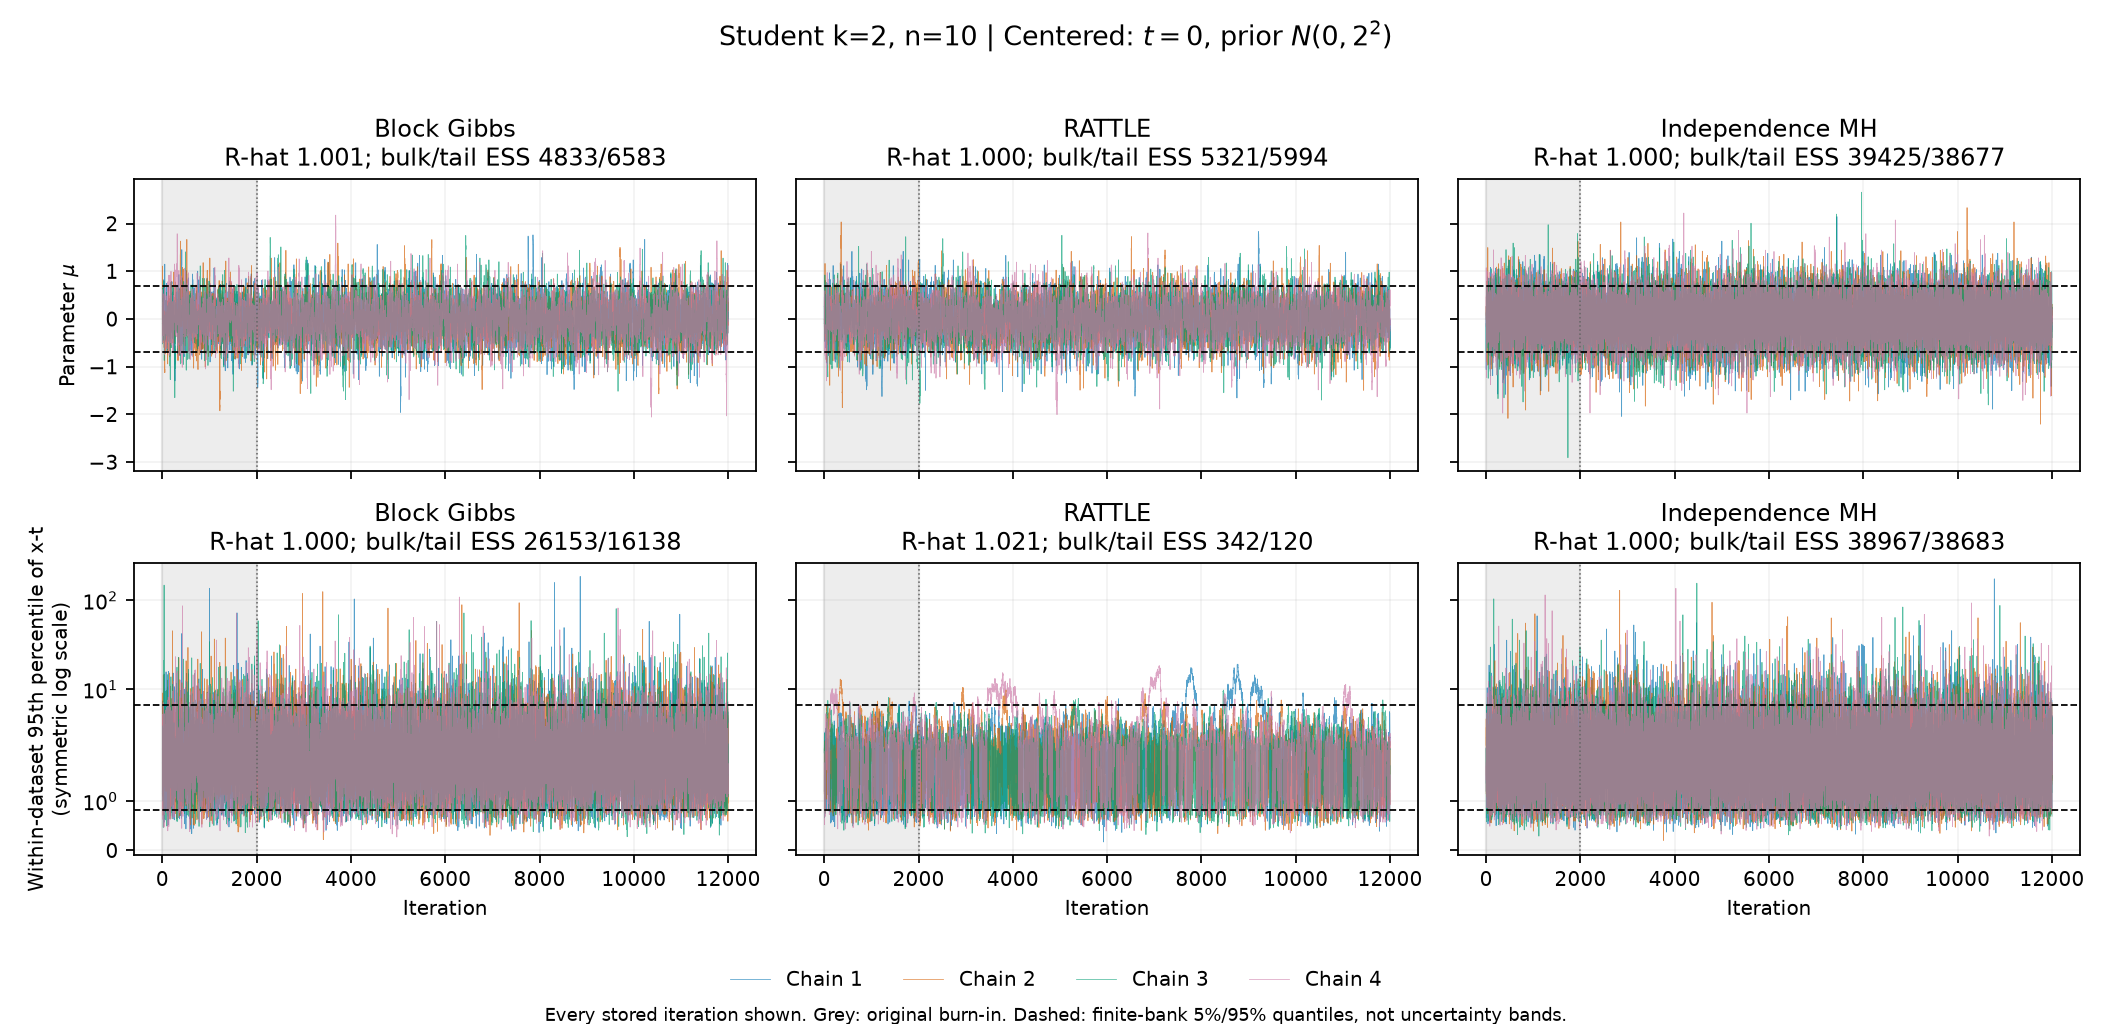
\includegraphics[keepaspectratio]{evidence/location_review_handoff_2026-10-12/figures/centered_n10.png}}
\caption{Centered Student parameter and upper latent-quantile traces}
\end{figure}

Centered n10 RATTLE has within-dataset Q95 R-hat 1.021 and tail ESS 120.
Its parameter trace would conceal this. Block and independence proposals
leave extreme configurations much more often.

\begin{figure}
\centering
\pandocbounded{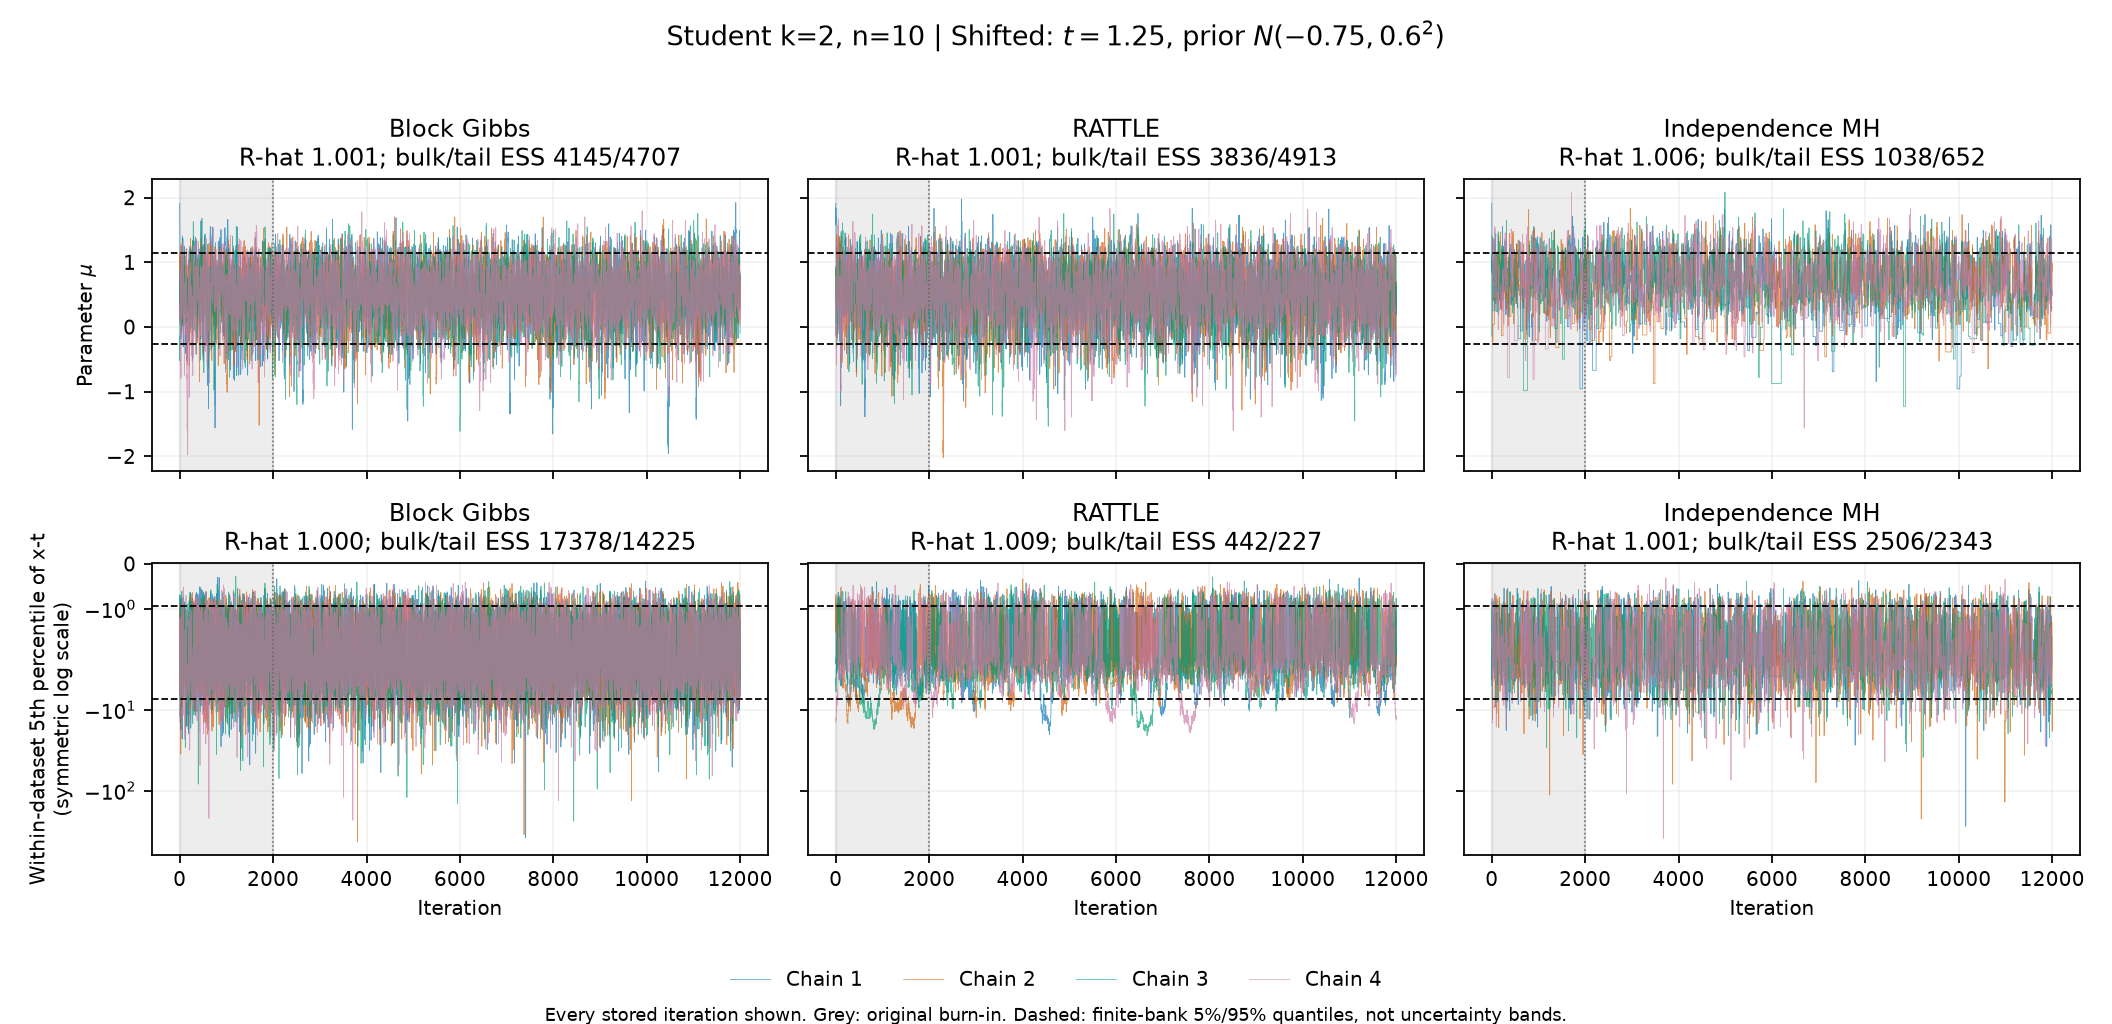
\includegraphics[keepaspectratio]{evidence/location_review_handoff_2026-10-12/figures/shifted_n10.png}}
\caption{Shifted Student parameter and lower latent-quantile traces}
\end{figure}

Shifted RATTLE's Q05 tail ESS is 227 even though R-hat is below 1.01.
Longest retained episodes with maximum residual above 6 are 630/404
iterations for centered/shifted RATTLE, versus 10/16 for block Gibbs.
RATTLE accepts 83.8--85.8\% and records no projection/reversal failures.
These observations point to slow transport at the tested settings, not a
high cost of selection or a proof of topological trapping. Student n3
RATTLE also misses a parameter quantile by 4.60 combined SEs and has
tail-event R-hat 1.0128.

Shifted independence MH passes the declared checks but has parameter
1\%-indicator ESS 323. Logistic n10 RATTLE passes symmetric summaries
while labelled coordinates reach R-hat 1.01585 and 1.01912. Shifted
Logistic block is borderline at 1.009988. Laplace passes labelled and
ordered checks; its fixed median is a constraint, not a converged random
observable. No failed run was extended or retuned.

\subsubsection{Cost in the same saved
benchmark}\label{cost-in-the-same-saved-benchmark}

Entries below are parameter-mean / latent-tail-event ESS per second. The
tail event is maximum residual above 6. Weighted MC reports
function-specific IID \textbf{equivalent} rates, not a count of
independent posterior draws.

\begin{longtable}[]{@{}
  >{\raggedright\arraybackslash}p{(\linewidth - 10\tabcolsep) * \real{0.1304}}
  >{\raggedleft\arraybackslash}p{(\linewidth - 10\tabcolsep) * \real{0.1739}}
  >{\raggedleft\arraybackslash}p{(\linewidth - 10\tabcolsep) * \real{0.1739}}
  >{\raggedleft\arraybackslash}p{(\linewidth - 10\tabcolsep) * \real{0.1739}}
  >{\raggedleft\arraybackslash}p{(\linewidth - 10\tabcolsep) * \real{0.1739}}
  >{\raggedleft\arraybackslash}p{(\linewidth - 10\tabcolsep) * \real{0.1739}}@{}}
\toprule\noalign{}
\begin{minipage}[b]{\linewidth}\raggedright
Case
\end{minipage} & \begin{minipage}[b]{\linewidth}\raggedleft
Block / median Gibbs
\end{minipage} & \begin{minipage}[b]{\linewidth}\raggedleft
RATTLE / facet HMC
\end{minipage} & \begin{minipage}[b]{\linewidth}\raggedleft
Independence MH
\end{minipage} & \begin{minipage}[b]{\linewidth}\raggedleft
Weighted MC
\end{minipage} & \begin{minipage}[b]{\linewidth}\raggedleft
Rejection draws/s
\end{minipage} \\
\midrule\noalign{}
\endhead
\bottomrule\noalign{}
\endlastfoot
Student n10 centered & 694 / 3,386 & 490 / 28\textdagger{} & 7,497 / 7,419 & 16,047
/ 15,172 & 14,820 \\
Student n10 shifted & 577 / 3,275 & 355 / 52\textdagger{} & 165 / 419 & 846 / 1,534
& 330 \\
Logistic n10 shifted & 1,894 / 10,886 & 487 / 188\textdagger{} & --- & 2,097 / 2,711
& 777 \\
Laplace n4 shifted & 2,630 / 30,528 & 766 / 548 & --- & 385,372 /
281,291 & 201,793 \\
\end{longtable}

\textdagger{} These runs fail expanded diagnostics and should not be ranked as
reliable joint posterior simulations. Burn-in and full direct-bank
generation costs are charged; compilation and analysis are excluded.
Timings are from the same saved study. Affine and transparent pair Gibbs
were not rerun and have no fresh speed ratio here. Vectorized Laplace
batches took only 3--5 ms, so publication-quality rate estimates need
longer timing batches. Rare-event uncertainty remains large when
independent rejection observes only a handful of events.

Direct methods are preferable for the tested centered cases and for
Laplace. Shifted Student rejection accepts only 2.17\%; block Gibbs is
useful for its latent tails. The n=3 certificate reduces block and
RATTLE full-selector calls to four each, one per chain, without curing
RATTLE's mixing. Faster validity checks alone will not solve that
transport problem.

\subsection{6. Review package and
reproducibility}\label{review-package-and-reproducibility}

Read this note first, then the
\href{location_only_performance_comparison.md}{performance report} and
the
\href{evidence/location_chain_diagnostics_2026-10-12/index.html}{full
trace gallery}. Use the linked target, kernel and geometry reports for
proofs and detailed tests. The gallery has 43 figures; the two figures
above are compact views made from the same saved chains, not new
experiments.

All 92 chains retain \texttt{mu} of shape \texttt{(12001,)} and
\texttt{x} of shape \texttt{(12001,n)}. Index zero is the initial state;
analysis uses \texttt{2001:} without thinning. The
\href{evidence/location_chain_diagnostics_2026-10-12/chain_inventory.csv}{chain
inventory} records seeds, shapes, ranges and hashes. The new
\href{evidence/location_review_handoff_2026-10-12/handoff_inventory.csv}{handoff
inventory} identifies source, reports and data, including untracked
source and Git-ignored banks. A Git commit or source zip alone does not
include this evidence.

The preservation record covers 1,824 pre-existing files. Only this note,
four entry guides and the manuscript status banner are edited. Previous
documents have a small recovery snapshot. Sampler/selector/reference
code, raw data and historical result manifests are unchanged. Current
checks and preservation results are in the
\href{evidence/location_review_handoff_2026-10-12/verification.json}{verification
record};
\href{evidence/location_review_handoff_2026-10-12/validation/}{validation
logs} record bounded tests, examples and CLI checks, including any
timeout or failure. The full existing suite passed \textbf{403 tests in
637.11 seconds} during this review. Both examples and all three CLI help
checks passed. There were no timeouts or collection failures. These
checks carry forward the saved scientific experiments; they do not rerun
or extend those experiments.

The inspected environment uses Python 3.13.5. Dependency bounds are not
a cross-platform certification. This host also uses the existing
isolated oracle dependencies at
\texttt{/tmp/student-mle-oracle-deps-20261003}. On another host, provide
the corresponding SymPy/mpmath dependencies rather than copying that
path. To regenerate only the two review figures, use a fresh
destination:

\begin{Shaded}
\begin{Highlighting}[]
\ExtensionTok{.venv/bin/python}\NormalTok{ scripts/build\_location\_review\_figures.py }\AttributeTok{{-}{-}out}\NormalTok{ tmp/review{-}figures{-}new}
\end{Highlighting}
\end{Shaded}

The \href{../../scripts/build_location_review_figures.py}{builder}
verifies input hashes and annotations and imports no sampler. Its
\href{evidence/location_review_handoff_2026-10-12/figures/provenance.json}{provenance
record} links both PNG/PDF outputs to the original inputs. For bounded
verification on this host:

\begin{Shaded}
\begin{Highlighting}[]
\FunctionTok{env}\NormalTok{ PYTHONPATH=/tmp/student{-}mle{-}oracle{-}deps{-}20261003 }\DataTypeTok{\textbackslash{}}
\NormalTok{  PYTEST\_DISABLE\_PLUGIN\_AUTOLOAD=1 PYTHONDONTWRITEBYTECODE=1 }\DataTypeTok{\textbackslash{}}
\NormalTok{  NUMBA\_CACHE\_DIR=/tmp/student{-}location{-}correctness{-}numba }\DataTypeTok{\textbackslash{}}
\NormalTok{  .venv/bin/python scripts/run\_checkpoint\_validation.py }\AttributeTok{{-}{-}out}\NormalTok{ tmp/review{-}checks{-}new}
\end{Highlighting}
\end{Shaded}

The runner uses one CPU and fixed time ceilings. Its two examples are
smoke checks, not convergence evidence. This documentation update starts
no new sampling study and does not change numerical defaults.

\subsection{7. Decisions for the
meeting}\label{decisions-for-the-meeting}

\begin{enumerate}
\def\labelenumi{\arabic{enumi}.}
\tightlist
\item
  \textbf{Scientific emphasis.} Agree whether the first manuscript
  should centre on the selected-statistic target, geometry and validated
  constructions. Claims about information loss or privacy need a
  separate defined question and evidence.
\item
  \textbf{Practical baseline.} Use raw weighting/rejection and block
  Gibbs as the present computational baselines. Decide whether a focused
  RATTLE transport investigation has enough scientific value before
  further speed work.
\item
  \textbf{Scope after review.} Review the known-scale theory and failure
  boundaries before wider n, singular/tie configurations or joint
  location-scale validation.
\end{enumerate}

We have a reviewable known-scale foundation. We do not yet have
universally certified selection, globally validated RATTLE mixing, or a
finished manuscript.

\end{document}
